% Version 2021
%

\chapter*{Datos de la Asignatura}
\label{chap:00.datos.de.IyA}
  \addcontentsline{toc}{chapter}{Datos de la Asignatura}

  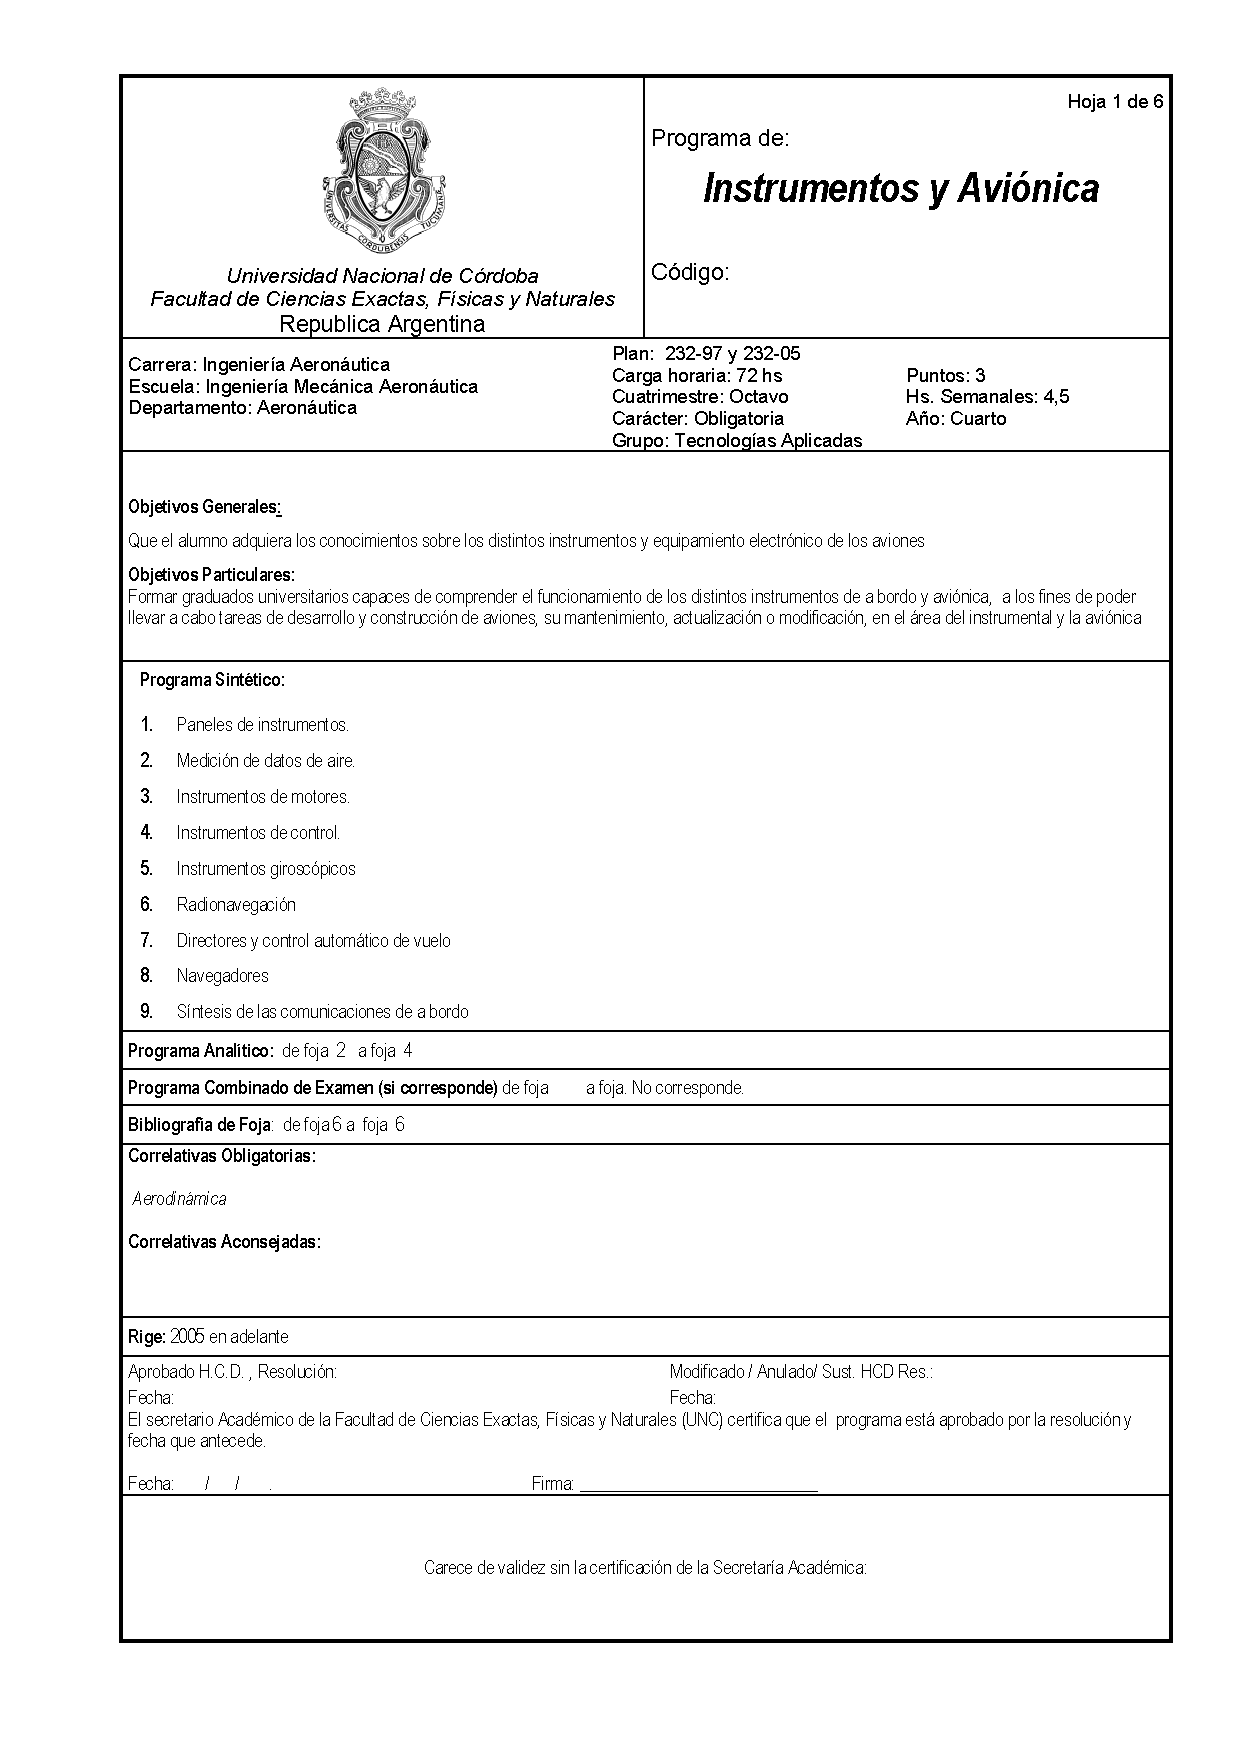
\includepdf[pages=-, fitpaper=false, scale=0.90, %landscape=true,
  offset = 0 -20,
  pagecommand={\thispagestyle{fancy}}]
  {00.Datos.IyA/Instrumentos_Y_Avionica.pdf}


\section{Días y horarios de clases}
\label{sec:dias+horarios.clases}

La asignatura se dicta de manera virtual en el año 2021
los días jueves de 17:30 hs a 22:00 hs.

Se emplea la plataforma Google Classroom.% el link a la misma es:

%\url{https://classroom.google.com/c/MzY3MDEyNzQ1MjA2?cjc=wbdwdwc}


\section*{Adecuación transitoria de la metodología de cursada  y evaluación segundo semestre 2021}
\label{00.Adecuacion.transitoria}
  \addcontentsline{toc}{section}{Adecuación transitoria de la metodología de cursada   y evaluación  segundo semestre 2021}


\subsection*{Modalidad de enseñanza virtual} 
Clases mediante google meet entre los docentes y los alumnos.
Material de estudio, asignación de tareas mediante Google Classroom
\subsection*{Modalidad de evaluación virtual}
Evaluación mediante Google Forms o mediante el envío de archivo .pdf con la evaluación que debe ser contestada por el alumno y reenviada al docente. Cantidad dos (2).

Las/los estudiantes que hayan desaprobado un (1) examen parcial teórico/práctico, si el restante examen parcial fue aprobado, tienen derecho a un (1) recuperatorio, cuya nota reemplazará a la del examen parcial reprobado.

Coloquio  tomados mediante google meet. Cantidad uno (1).

\subsection*{Condiciones Transitorias de Regularidad}

\begin{itemize}
\item Estar correctamente matriculado para el cursado de la asignatura
\item Aprobar con nota no inferior a 4 (cuatro), uno (1) de los dos
  (2) exámenes parciales.
\item Aprobar un coloquio integrador con nota no inferior a 4 (cuatro)
\item Presentar y aprobar los trabajos prácticos
\end{itemize}

\subsection*{Condiciones Transitorias de Aprobación definitiva (Promoción) }


\begin{itemize}
\item Haber aprobado las correlativas previas o aprobar las que se encuentren pendientes dentro del plazo de validez de la regularidad.

\item  Estar correctamente matriculado para el cursado de la
  asignatura
\item Aprobar con nota no inferior a 4 (cuatro) los dos (2) exámenes
  parciales.
\item Aprobar un coloquio integrador con nota no inferior a 4 (cuatro)
\item Presentar y aprobar los trabajos prácticos
\end{itemize}



\section*{Cronograma para el dictado de la Asignatura a\~no 2021}
\label{sec:00.cronograma}
  \addcontentsline{toc}{section}{Cronograma para el dictado a\~no 2021}

  \begin{itemize}
  \item Capítulo 1. Paneles de Instrumentos (García) 5/8/21
  \item Capítulo 2. Medición de datos de aire (Galeasso) 12/8/21
  \item Capítulo 4. Instrumentos de control. 
        Capítulo 3. Instrumentos de motores (Giraudo) 19/8/21
  \item Capítulo 5. Instrumentos giroscópicos (Galeasso) 26/8/21
  \item \textbf{Parcial 01,  2/9/2021 Abarca Capítulos 1, 2,3, 4 y 5}

  \item Capítulo 6. Radionavegación (Garcia) 9/9/21
  \item Capítulo 7. Directores y control automático de vuelo ( García)     16/9/21
  \item Capítulo 8. Navegadores (Garcia) 23/9/21
  \item Capítulo 8. Navegadores (GPS, nav. inerc.) (Giraudo) 7/10/21
  \item Capítulo 9. Síntesis de las comunicaciones de a bordo (Garcia)     14/10/21

  \item {\bf Parcial 02,  21/10/2021 Abarca Capítulos 6, 7, 8 y 9}
  \item \textbf{Recuperatorios Parciales. Entrega de Trabajos Prácticos. 28/10/2021}

  \item \textbf{Coloquio,  4/11/2021 Abarca todo el programa}
  \item \textbf{Coloquio, 11/11/2021 Abarca todo el programa}
  \end{itemize}


\section*{Docentes}
\label{00.docentes}
  \addcontentsline{toc}{section}{Docentes}

  \begin{tabular}{llm{0.5\textwidth}} \rowcolor{yellow!30}
 {\bf Docente} & {\bf Correo electr\'onico} & {\bf D\'ia, horario consulta, medio de consulta} \\ \rowcolor{cyan!20}
  Ing. Jorge Garcia & jgarcia@unc.edu.ar & D\'ia Mi\'ercoles, de 15 a 17 hs, correo electr\'onico, google meet \\ 
  Ing. Angel Galeasso & angel.galeasso@unc.edu.ar & D\'ia Mi\'ercoles, de 16 a 17 hs, correo electr\'onico, google meet    \\ \rowcolor{cyan!20} 
  Ing. Pedro Giraudo  & pedrogiraudo@unc.edu.ar &  D\'ia Mi\'ercoles, de 17:30 a 19 hs, correo electr\'onico, google meet, zoom     \\
\end{tabular}